
\newpage\subsection*{Άσκηση 1}

Κάθε γράφημα $G$ χωρίς βρόγχους έχει διμερές υπογράφημα $H \subseteq G$ με τουλάχιστον 
$|E(G)|/2$ ακμές (Δείτε σελ. 29 των σημειώσεων για την απόδειξη της πρότασης αυτής). 
Εφαρμόστε την κατασκευή της απόδειξης στο παρακάτω 6-κανονικό γράφημα $G$ με 13
κορυφές και βρείτε ένα διμερές επαγόμενο υπογράφημα με τουλάχιστον $|E(G)|/2$ ακμές.
Ξεκινήστε με τα εξής σύνολα διαμέρισης: $V_1 = \{v_{13}\}$ και $V_2 = \{v_1,...,v_{12}\}$.

\begin{center}
    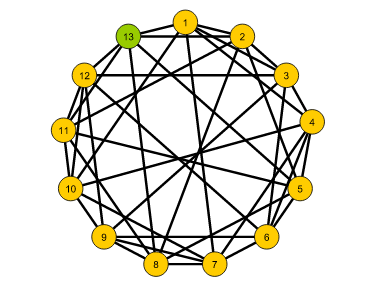
\includegraphics[width=.4\textwidth]{./exercise1/Selection_002.png}
\end{center}

\subsubsection*{Λύση}

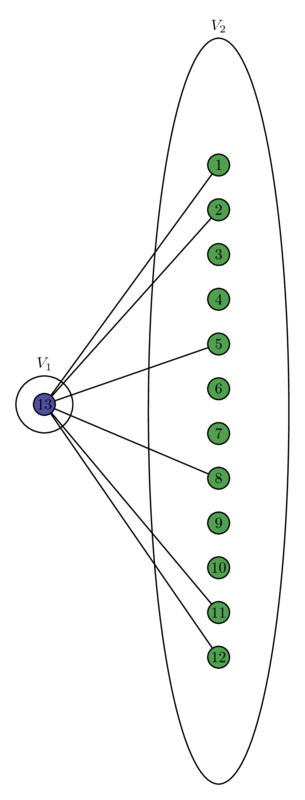
\includegraphics[height=10cm,width=.24\textwidth]{./exercise1/diagrams/test4.png}
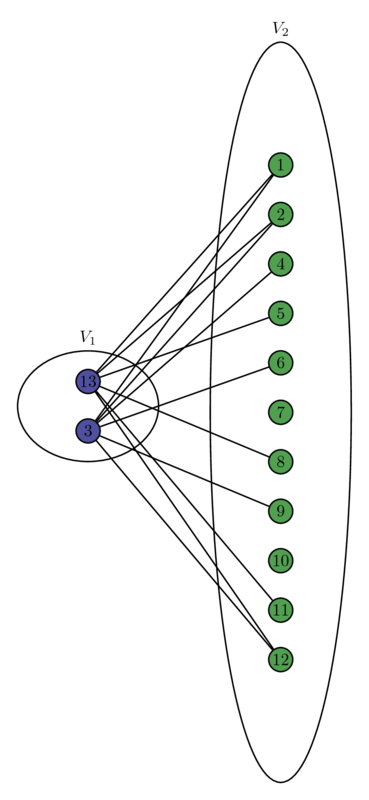
\includegraphics[height=10cm,width=.24\textwidth]{./exercise1/diagrams/test5.png}
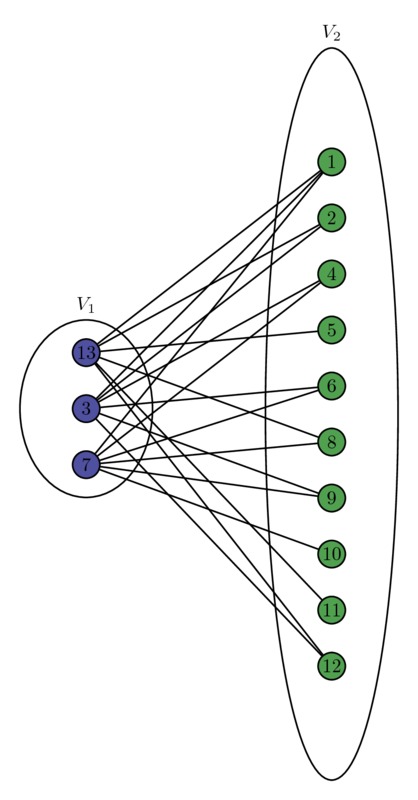
\includegraphics[height=10cm,width=.24\textwidth]{./exercise1/diagrams/test6.png}
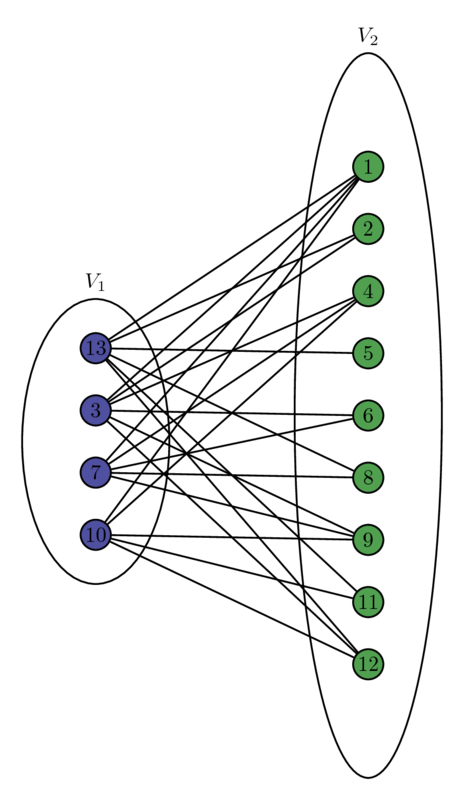
\includegraphics[height=10cm,width=.24\textwidth]{./exercise1/diagrams/test7.png}


